\chapter{Návrh}

V této kapitole popíšeme návrh realizace požadavků, které jsme uvedli v kapitole analýza.

\section{Architektura aplikace}

Aplikace se bude skládat ze tří částí; dvou těsně provázaných (serverová, klientská) a jedné volitelné (doplněk do prohlížeče).

Celek tvořený serverovou a klientskou části bude rozdělen do několika vrstev podle konceptu \zkratka{MVP}{Model-view-presenter -- členění aplikace na tři části, kde každá je zodpovědná za jednu úlohu: model reprezentuje data, view zobrazuje data, presenter předává požadavky uživatele a vrací výsledná data}.

\subsection{Serverová část}

Serverovou část postavíme na platformě Google AppEngine; využijeme mnoho možností, které nabízí.
Pro realizaci některých specifických částí použijeme volně dostupné knihovny.

Serverová část bude obsahovat vrstvu modelu a prezentéra.

\subsubsection{Úloha serverové části}

Serverová část bude mít v aplikaci následující úlohy:
\begin{itemize}
	\item uložení všech dat,
	\item poskytování dat klientům,
	\item periodický sběr nových položek kontrolou zdrojů,
	\item výpočet doporučení zdrojů klientům na základě podobnosti.
\end{itemize}

\subsubsection{Uložení dat}

Všechna data, jak sdílená, tak i dedikovaná jednotlivým uživatelům, budeme ukládat do databáze Datastore, kterou poskytuje platforma AppEngine.
Data budou modelována s pomocí frameworku Slim3, který použijeme jako obálku kolem samotné databáze.
K vlastním datům v databázi budeme přistupovat pomocí sady služeb zaměřených podle typu objektů, se kterými pracují.

\subsubsection{Rozhraní služeb}

Pro komunikaci s klientskou částí navrhneme sadu rozhraní/služeb, přes která bude probíhat veškerá komunikace.
Realizaci vlastní komunikace přenecháme frameworku GWT za účasti knihovny Slim3.
Tyto služby budou mít za úkol kontrolovat požadavky klientů a volat příslušné služby komunikující přímo s databází.

\subsubsection{Služby pro realizaci procesů}

Naše aplikace bude vykonávat několik náročnějších procesů; mezi ně patří kontrola zdrojů, zálohování a výpočet doporučení.

\paragraph{Kontrola zdroje}
Při kontrole zdrojů využijeme frontu úloh -- pro každý požadavek na kontrolu zdroje vytvoříme úlohu.
Úloha kontroly zdrojů vyžaduje stažení dokumentu z webu: buď HTML, nebo XML.
Pro stažení použijeme knihovnu HttpComponents.

Pokud je zdroj typu RSS/Atom, použijeme knihovnu ROME pro rozparsování dokumentu.
Pokud naopak zdroj pracuje s webovými stránkami, vytvoříme pomocí knihovny jsoup její stromovou reprezentaci, se kterou budeme dále pracovat.
V případě, že zdroj je typu Změna stránky, použijeme knihovnu Diff Match Patch pro výpočet, určení změny.

\paragraph{Zálohování položky}
Při zálohování položky musíme nejprve stáhnout webovou stránku kterou reprezentuje; využijeme opět knihovnu HttpComponents.
Strán\-ku následně upravíme (změníme všechny relativní odkazy a cesty k obrázkům) převedením do DOMu pomocí knihovny jsoup a provedením vhodných operací s elementy.
Upravenou stránku uložíme do \uv{souboru} pomocí rozhraní poskytovaného službou Google Cloud Storage.

Zálohovanou stránku budeme poskytovat pomocí metod služby Blobstore, které nám umožní její přímé streamování.

\paragraph{Exportování položek}
Knihovnu ROME použijeme i pro opačný směr konverze, využijeme její generátory pro tvorbu RSS a Atom dokumentů při sdílení (exportu) položek.

\paragraph{Výpočet doporučení}
Algoritmus pro výpočet doporučení je realizovatelný posloupností operací provedených nad maticemi.
Použijeme modul lineární algebry z knihovny JScience k výpočtům s vektory a maticemi.

\subsection{Klientská část}

Klientskou část uvidí uživatel při každé návštěvě webové stránky aplikace.
Je tvořena drobnou kostrou napsanou v HTML, která je masivně rozšířená \pojem[JavaScriptovým]{JavaScript}{formálně ECMAScript, interpretovaný jazyk běžící v internetovém prohlížeči, který umožňuje tvůrci webové stránky interaktivně manipulovat s jejím obsah} frameworkem, který zajišťuje dynamičnost a interaktivitu celé stránky.
Vzhled stránky je definovaný v jazyku CSS.

Klientská část bude obsahovat vrstvu prezentéra a zobrazení.

\subsubsection{Úloha klientské části}

Uživatel ovládá celou aplikaci klientskou částí pomocí prvků grafického prostředí webové stránky.
Přes ní manipuluje se všemi svými daty uloženými v serverové části aplikace.
Mezi nejdůležitější úkony prováděné uživatelem patří:
\begin{itemize}
	\item správa zdrojů: přidání a úprava zdroje, zastavení a obnovení sledování zdroje
	\item procházení seznamu položek, zobrazení originálu položky, přidání/odebrání štítku, zazálohování položky
	\item filtrování seznamu položek, změna kritérií filtru, správa filtrů
	\item nastavení ostatních vlastností aplikace
\end{itemize}

Jelikož serverová část aplikace bude vytvořena v jazyku Java, zvolili jsme pro vývoj klientské části nástroj, který umožňuje zkompilovat kód v jazyku Java do jazyku JavaScript.
Tímto nástrojem je GWT.

Samotné knihovny GWT obsahují mnoho užitečných grafických prvků, nic\-mé\-ně neobsahují například dialog pro výběr barev.
GWT Eye Candy je knihovna, která nám rozšíří nabídku grafických komponent.
My z ní využijeme jediný prvek: ColorPicker pro výběr barvy štítků.

\subsection{Doplněk do prohlížeče}

Nepovinný doplněk má za úkol zvýšit komfort používání aplikace těm uživatelům, kteří mají možnost instalace doplňků do prohlížeče.

\subsubsection{Funkce doplňku}

Doplněk slouží k přidání nové manuální položky do aplikace.
Doplněk bude mít podobu tlačítka na liště v prohlížeči; kliknutím na tlačítko se objeví vyskakovací okno s předvyplněnou adresou a titulkem aktuální stránky.
V případě, že uživatel vybral část textu na stránce, bude jím předvyplněn popis položky.
Kliknutím na tlačítko \uv{Odeslat} se vytvoří v aplikaci nová manuální položka podle vyplněných údajů.

\bigskip

Doplněk vytvoříme na platformě Crossrider, která zajistí produkci výsledných doplňků do nejběžnějších prohlížečů.
Z možností platformy využijeme jen zobrazení tlačítka v liště prohlížeče, komunikaci po síti, databázi k uložení hodnot a posílání zprav mezi jednotlivými částmi doplňku.

Nejdůležitější částí doplňku je popup okno, zobrazené po kliknutí na tlačítko; obsah tohoto okna je běžná webová stránka, která bude obsahovat formulář s údaji o položce.
Součástí formuláře je i seznam štítků, který budeme realizovat knihovnou TexExt, která bude poskytovat uživatelsky přívětivé rozhraní.

\section{Entity}

Entity jsou obecné struktury, se kterými aplikace pracuje.
Cílem této kapitoly je entity popsat a vysvětlit úlohu, kterou mají v kontextu celé aplikace.
Pro přehlednost jsme entity sdružili do oblastí, jichž se týkají.

\subsection{Uživatele a konfigurace}

Oblasti uživatele a konfigurace obsahuje následující entity.

\subsubsection{Uživatel}

Uživatel je reprezentace osoby, která systém používá.
Entitu uživatele přebíráme od poskytovatele serveru pomocí Users API.

\subsubsection{Konfigurační položka}

Konfigurační položka nemá nic společného s termínem položka ani entitou položka.

Jedna konfigurační položka definuje jeden parametr, který má vliv na vzhled nebo chování aplikace; lze rozlišit dva typy konfiguračních položek:
\begin{itemize}
	\item konfigurace serverové části -- závisí na ní chování serverové části,
	\item konfigurace klientské části -- závisí na ní vzhled nebo chování klientské části.
		Hodnoty položek tohoto typu mohou záviset na konkrétním uživateli, který aplikaci používá.
\end{itemize}

\subsection{Zdroje}

Tato část seskupuje všechny entity, které souvisejí se zdroji položek, jejich reprezentací a zpracováním.
Nejdůležitější dvojicí entit je zdroj a uživatelský zdroj: zdroj má význam pouze pro pravidelné kontroly existence nových položek, uživatelský zdroj popisuje zdroj z pohledu uživatele.
Oblast zdrojů obsahuje tyto entity:

\subsubsection{Zdroj}
\label{sss:zdroj}

Zdroj reprezentuje každou webovou stránku nebo službu, kterou aplikace používá k získávání nových položek.
Aplikace pravidelně kontroluje změny na zdrojích; pokud zaregistruje změnu, aplikace přidá odpovídající položky.
Zdroj je abstraktní entita, od které jsou odvozeny jednotlivé typy zdrojů; obsahuje všechny informace nutné k tomu, aby zdroj mohl být periodicky kontrolován.
Typy zdrojů jsou:

\paragraph{Manuální zdroj}

Manuální zdroj patří vždy jednomu konkrétnímu uživateli.
Nereprezentuje žádnou internetovou adresu a sám o sobě neposkytuje žádné položky.
Všechny položky, které tomuto zdroji patří, přidal sám uživatel pomocí některé ze služeb, které má k dispozici.
Jde tedy o technický prostředek, jak naplnit funkcionalitu přidávání vlastních položek.

\paragraph{RSS/Atom}

RSS a Atom jsou formáty XML dokumentů, které popisují novinky, ke kterým došlo za poslední dobu na webovém portálu.
Tento zdroj typicky obsahuje odkazy na články, které byly publikovány v nedávné minulosti.

\paragraph{Webový rozcestník}

Nahrazuje funkcionalitu RSS či Atom pro webové portály, které tyto kanály neposkytují.
Vychází z jednoduchého pozorování, že úvodní stránka takového portálu obsahuje seznam nejnovějších článků a že položky převzaté z RSS či Atomu by odpovídaly odkazům na této stránce.

\paragraph{Změna stránky}

Reprezentuje webovou stránku, o jejíž změně obsahu chce být uživatel informován.
Každá změna stránky způsobí vytvoření položky informující o změně.

\subsubsection{Region}

Region definuje pro typ zdroje Webový rozcestník a Změna stránky oblast stránky, která je z pohledu uživatele zajímavá.
Region je určen výběrem oblastí stránky, které se mají kontrolovat a oblastí, které se mají při kontrole ignorovat.
Motivací k pozitivnímu a negativnímu přístupu k jednotlivým částem je fakt, že stránky obsahují prvky, který se mění při každém dotazu (reklamy, informace o času generování stránky) nebo není zajímavý (hlavička a patička stránky, menu).

\subsubsection{Uživatelský zdroj}
\label{sss:uzivatelsky-zdroj}

Zavedeme entitu uživatelský zdroj, jež realizuje vztah mezi uživateli a zdroji.
Několik uživatelů může sledovat stejný zdroj a každý uživatel většinou sleduje více zdrojů.
Tato entita uchovává vlastní nastavení každého zdroje zvlášť pro každého uživatele.
Počet aktivních uživatelských zdrojů určuje, politiku podle které bude probíhat jeho kontrola.
Uživatel vždy pracuje s uživatelskými zdroji, od zdrojů, které jsou pod nimi, je odstíněn.
Pokud je v uživatelském rozhraní zmíněn pojem zdroj, je jím myšlena tato entita; entita zdroje nemá pro uživatele praktický význam.

Uživatelský zdroj obsahuje entitu štítek, která reprezentuje informaci o příslušnosti položky ke zdroji.
Této nepřímé vazby využíváme v dotazech do databáze, při kterých klademe na uživatelské položky kritérium, že musejí pocházet z konkrétního uživatelského zdroje.
Více o tomto štítku a jeho funkci popíšeme v kapitole~\ref{sss:stitek}.

\subsection{Položky}

Oblast položek obsahuje následující entity.

\subsubsection{Položka}

Položkou v aplikaci myslíme jednu adresu webové stránky, která pochází z některého ze zdrojů nebo byla přidána uživatelem manuálně.
Položka je závislá jen na zdroji, ze kterého pochází, vlastní personalizaci (přizpůsobení jednotlivým uživatelům) se zabývá entita uživatelská položka.
Každý typ zdroje poskytuje položky jiného typu:

\paragraph{Manuální položka}

Manuální položka formálně patří k manuálnímu zdroji; jediným důvodem je zajištění konzistence rozhraní všech typů položek.
Manuální položka reprezentuje libovolnou internetovou adresu spolu s titulkem a popisem.
Manuální položka vzniká jen a pouze činností uživatele, který si ji sám přidá do aplikace.
Motivací zavést manuální položku je umožnění uživateli:
\begin{itemize}
	\item přidat vlastní informaci k libovolné stránce,
	\item zazálohovat libovolnou stránku,
	\item označit si libovolnou stránku k pozdějšímu přečtení.
\end{itemize}

\paragraph{Položka typu článek}

Položka typu článek je produkována při kontrole zdrojem typu RSS/Atom.
Každému záznamu v XML dokumentu odpovídá jedna položka vytvořená v aplikaci při kontrole zdroje.
Titulek a popis přebíráme spolu s dalšími informacemi přímo z RSS/Atom dokumentu.
Položka typu článek může poskytovat více informací než jiné typy položek: jedná se především o jméno autora článku a datum publikace.
Obecně tyto informace nejsou jednoduše zjistitelné v případě položek jiných typů.

\paragraph{Položka typu odkaz}

Položka typu odkaz pochází ze zdroje typu webový rozcestník.
Každému nalezenému odkazu na webové stránce (uvnitř regionem omezené oblasti) odpovídá právě jediná položka.
Titulek resp. popis přebíráme z textu odkazu resp. textu nejbližšího okolí odkazu.

\paragraph{Položka typu změna stránky}

Položka typu změna stránky pochází ze zdroje typu změna stránky.
Při kontrole stránky (na kterou se odkazuje zdroj) se porovnává její textový obsah s verzí, kterou jsme si uložili při předchozí kontrole.
Pokud je nalezena změna, aplikace vytvoří novou položku, která bude obsahovat popis změn stránky.

\bigskip

Položka je závislá jen na zdroji, ze kterého pochází; stejně jako v oblasti zdrojů existuje dvojice: zdroj -- uživatelský zdroj, existuje i entita uživatelská položka.

\subsubsection{Uživatelská položka}

Entita položka obsahuje jen obecné -- na uživateli nezávislé atributy, které jsou sdíleny všemi uživateli.
Jsou jimi například: titulek, obsah, zdroj, ze kterého pochází, datum a čas přidání.
Aby mohl každý uživatel mít položku ve vlastním stavu, s vlastními štítky, zavedeme entitu uživatelská položka.
Tato entita uchovává nastavení vlastní každému uživateli, včetně zálohy, pokud byla vytvořena.

Pokud je v uživatelském rozhraní zmíněn pojem položka, je jím myšlena tato entita; entita položka nemá pro uživatele praktický význam.

\bigskip

Na obrázku~\ref{fig:source-item} je zobrazen vztah nejdůležitějších entit z oblastí zdrojů a položek.

\begin{figure}
    \centering
    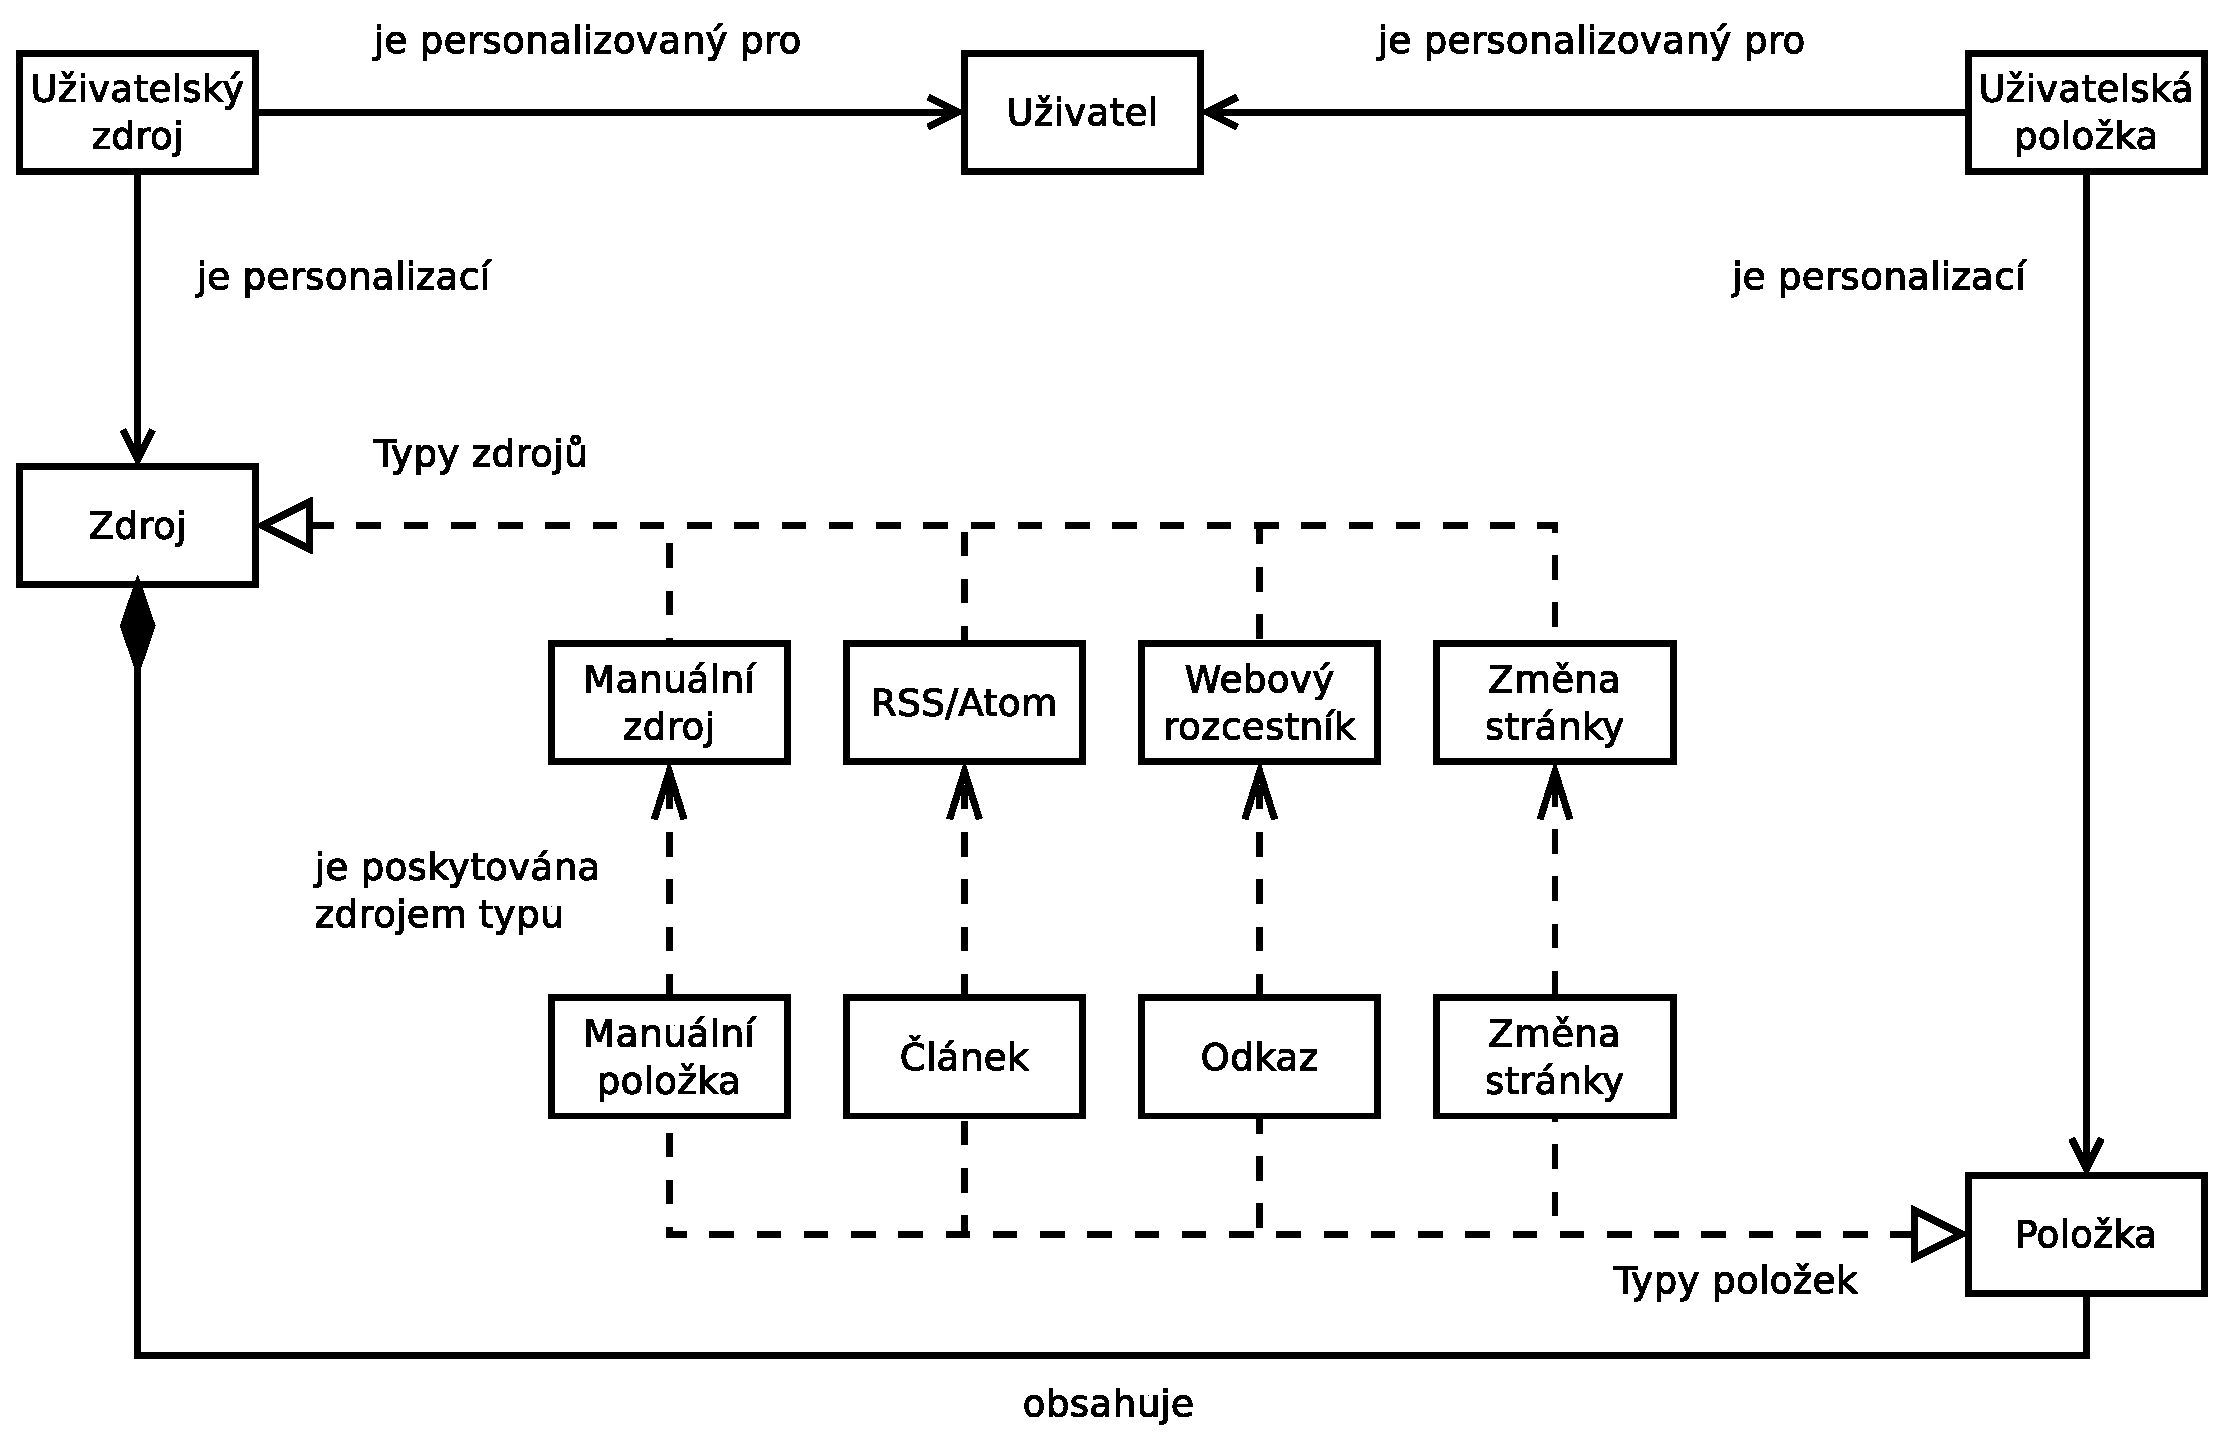
\includegraphics[width=14cm]{zdroje-polozky.eps}
    \caption{Vztahy mezi uživatelem, zdroji a položkami}
    \label{fig:source-item}
\end{figure}

\subsection{Štítky}

\subsubsection{Seznam položek}
Než zavedeme entity této oblasti, zadefinujeme pojem seznam položek.

Seznam (uživatelských) položek je podle času vzestupně či sestupně uspořádaný seznam všech uživatelských položek, které vyhovují všem kritériím, které jsou uživatelem na seznam kladeny.
Seznam položek je výsledkem dotazu, neexistuje dokud není dotaz proveden.

Termín seznam položek používáme také pro komponentu grafického prostředí, která zobrazuje uživatelské položky, které jsou součástí seznamu položek, výsledku dotazu.

Oblast štítků obsahuje následující entity.

\subsubsection{Štítek}
\label{sss:stitek}

Štítek reprezentuje informaci, kterou může uživatel přidat ke své uživatelské položce.
Štítek má svého vlastníka, uživatele, který jej vytvořil; tento štítek není dostupný jiným uživatelům.
Štítek má několik úloh:
\begin{itemize}
	\item tvoří poznámku u uživatelské položky,
	\item lze filtrovat uživatelské položky mající přiřazený konkrétní štítek,
	\item přiřazením vhodného štítku k uživatelské položce se provede záloha webové stránky položky.
\end{itemize}

Abychom zajistili jednoduché používání štítků, zavedli jsme následující dvě omezení:
\begin{itemize}
	\item Název štítku nesmí obsahovat bílé znaky a znak \$.
		Bílé znaky na okrajích názvu se oříznou, bílé znaky uvnitř a znak \$ způsobí chybu při vytváření/přiřazování štítku.
		Toto omezení vynucuje výstižná jednoslovná pojmenování štítků.
	\item Název štítku nelze později změnit.
		Toto omezení umožňuje využít název štítku jako část jeho klíče.
\end{itemize}

V aplikaci existují dva typy štítků:
\begin{enumerate}
	\item uživatelský štítek -- štítek, který vytvořil uživatel, je přiřazovaný uživatelem a je zobrazovaný v seznamu položek,
	\item zdrojový štítek -- štítek reprezentující uživatelský zdroj -- tento typ štítku není spravován uživatelem, nemůže jej ani vytvořit ani přiřadit, nezobrazuje se v seznamu položek.
		Jde o technickou záležitost, která nám umožňuje zjednodušit některé dotazy do databáze.
\end{enumerate}

\paragraph{Seznam štítků u uživatelských zdrojů}
Uživatel má možnost u svého uživatelského zdroje uvést seznam štítků, které mají být automaticky přidány ke každé uživatelské položce, která patří danému uživatelskému zdroji.
V případě, že zdroj je typu manuální zdroj, nebudou štítky přidány k uživatelské položce automaticky, ale budou jen uživateli nabídnuty přednostně.

Každý uživatelský zdroj obsahuje právě jeden zdrojový štítek; tento štítek zároveň patří právě jednomu uživatelskému zdroji a je vždy součástí zmíněného seznamu štítků.

Můžeme říct, že existuje dvojí vazba mezi uživatelským zdrojem a jeho uživatelskými položkami:
\begin{enumerate}
	\item přímá vazba uživatelské položky na uživatelský zdroj;
	\item nepřímá vazba přes společný zdrojový štítek.
		Tuto vazbu využijeme dále při popisu entity seznamový filtr.
\end{enumerate}

\subsubsection{Seznamový filtr}

Seznamový filtr popisuje kritéria a způsob řazení seznamu položek.
Řazení je vždy buď sestupně či vzestupně podle času přidání uživatelské položky.
Možná kritéria jsou následujících typů:
\begin{itemize}
	\item přečtená/nepřečtená uživatelská položka,
	\item nejstarší/nejnovější datum přidání uživatelské položky,
	\item filtr tvořený predikáty: \uv{Uživatelská položka $X$ má přiřazený štítek $Y$}
\end{itemize}

Poslední uvedené kritérium je zásadní pro funkčnost celé aplikace a všech seznamů položek:
\begin{itemize}
	\item seznam všech položek -- filtr je prázdný
	\item položky mající konkrétní štítek -- filtr obsahuje právě ten štítek,
	\item položky konkrétního uživatelského zdroje -- filtr obsahuje štítek patřící uživatelskému zdroji,
	\item složitější filtry -- předchozí dvě možnosti spojené pomocí operátorů \verb|AND| a \verb|OR|\footnote{Databáze má stanovené omezení na složitost dotazu: dotaz může obsahovat maximálně 30 větví disjunkce.}.
\end{itemize}

\paragraph{Typy filtrů}
V rámci aplikace rozlišujeme tři typy seznamových filtrů.
\begin{itemize}
	\item obyčejný seznamový filtr -- seznamový filtr, který si uživatel uložil a kdykoli si může zobrazit seznam položek, které mu vyhovují,
	\item exportovaný seznamový filtr -- chová se shodně jako obyčejný seznamový filtr; umožňuje navíc zobrazit seznam položek jako RSS či Atom dokument komukoli mimo naši aplikaci,
	\item ad-hoc seznamový filtr -- slouží pro okamžitou navigaci mezi různými seznamy položek v aplikaci, není trvale uložený.
		Ad-hoc seznamovým filtrem je například realizován seznam položek zobrazený po kliknutí na libovolný štítek.
\end{itemize}

\subsection{Klávesové zkratky}

V aplikaci existuje jediná entita, která popisuje klávesové zkratky.

\subsubsection{Klávesová zkratka}

Klávesová zkratka definuje chování aplikace, které nastane při stisku klávesy či kláves.
Každý uživatel si může definovat svoji vlastní sadu klávesových zkratek.
Rozlišujeme tři různé typy klávesových zkratek:
\begin{itemize}
	\item zkratky, které přiřazují či odebírají štítky uživatelským položkám.
		Klávesová zkratka má vazbu na štítek, který se má k uživatelské položce přidat, pokud přiřazen není, či odebrat, pokud je již přiřazen.
	\item zkratky, které zobrazují seznam položek.
		Klávesová zkratka má vazbu na seznamový filtr, který se má použít pro zobrazení seznamu položek.
	\item zkratky, které vykonávají jednu z mnoha podporovaných akcí.
		Takovou akcí může být například přechod na následující položku, zrušení aktuálního filtru či zobrazení originální stránky položky.
\end{itemize}

\section{Procesy}

Na tomto místě popíšeme procesy, které manipulují s entitami.
Z popsaných procesů je zřejmé, jak jsou jimi realizovány jednotlivé funkční požadavky na aplikaci.

\subsection{Zdroje}

Po přihlášení si uživatel může vytvořit své vlastní zdroje:
\begin{enumerate}
	\item zjistí se, zda takový zdroj již existuje (URL a typ zdroje),
	\item pokud neexistuje vytvoří se nový zdroj příslušného typu,
	\item vytvoří se uživatelský zdroj, který propojí zdroj s uživatelem.
\end{enumerate}

Uživatel nebude moci vytvořit zdroj typu manuální zdroj; manuální zdroj se vytvoří automaticky při prvním přihlášení.
Při každém přihlášení se zkontroluje, zda existuje; pokud neexistuje, vytvoří se výše uvedeným postupem.

Odstranění zdroje není možné z důvodu, že mohou existovat položky, které jsou na tento zdroj navázané.
Uživatel může zrušit sledování zdroje změnou vlastnosti uživatelského zdroje; sledování zdroje může uživatel obnovit.
Pokud bylo u zdroje zrušeno sledování, nebudou se nadále vytvářet uživatelské položky pro tento uživatelský zdroj.
V případě, že neexistuje aktivní uživatelský zdroj pro zdroj, nebude se provádět jeho kontrola.
K tomu může dojít dvěma způsoby:
\begin{itemize}
	\item buď uživatel zrušil sledování zdroje,
	\item nebo během vytváření uživatelského zdroje byl objeven chybně zadaný údaj.
\end{itemize}

\subsection{Položky}

Aplikace pravidelně provádí kontrolu zdrojů; stáhne z internetu dokument odpovídající adrese zdroje a zpracuje jej.
Pokud se při kontrole zdroje zjistí, že záznam ještě v aplikaci neexistuje, bude vytvořen.
\begin{enumerate}
	\item Vytvoří se položka podle typu zdroje,
	\item zjistí se z databáze seznam všech aktivních uživatelských zdrojů pro daný zdroj,
	\item vytvoří se nová uživatelská položka pro každý aktivní uživatelský zdroj.
\end{enumerate}

Uživatel může do aplikace přidat webovou stránku jako novou položku.
V případě, že uživatel přidává položku manuálně:
\begin{enumerate}
	\item nalezne se uživatelský zdroj odpovídající uživatelovu manuálnímu zdroji,
	\item vytvoří se manuální položka pro manuální zdroj nalezeného uživatelského zdroje,
	\item vytvoří se uživatelská položka pro nalezený uživatelský zdroj.
\end{enumerate}

\subsection{Seznamy položek}

Seznam položek je definován seznamovým filtrem -- několika kritérii, kterým musí každá položka vyhovět.
Ad-hoc seznamový filtr vzniká v aplikaci přirozeně akcemi uživatele, je jím realizován například výpis položek uživatelského zdroje.
Uživatel může zobrazit seznam položek na základě svého ad-hoc seznamového filtru; takový seznamový filtr může dále pojmenovat a uložit.
Uživatel si může zadefinovat libovolné množství vlastních seznamových filtrů, přeneseně i seznamů položek.
Seznamový filtr může dále měnit, případně odstranit.

\subsection{Štítky}\label{ssec:procesy-stitky}

Uživatel má možnost přidat k položce dodatečnou informaci prostřednictvím štítku; přidání štítku může probíhat i polo-automaticky (klávesovou zkratkou) či plně automaticky (uvedením štítku do seznamu automaticky přidávaných štítku v uživatelském zdroji).

Uživatel může na několika místech vybrat štítek ze seznamu existujících štítků, případně vytvořit nový, pokud žádaný štítek ještě neexistuje.
Štítek lze odstranit, za předpokladu, že není nikde v aplikaci použit: položkou, seznamovým filtrem, či klávesovou zkratkou.

Pokud má štítek nastavenou vlastnost zálohování, jeho přiřazení uživatelské položce způsobí zazálohování webové stránky položky:
\begin{enumerate}
	\item stáhne se webová stránka položky,
	\item veškeré relativní odkazy na stránce se nahradí za absolutní,
	\item uloží se soubor stránky do úložiště pomocí služby Google Cloud Storage a zapíše klíč do uživatelské položky.
\end{enumerate}

\subsection{Klávesové zkratky}

Uživatel si může přiřadit klávesové zkratky k nejběžnějším úkonům.
Klávesovou zkratku vytvoří uvedením klávesy či kombinace kláves, které spustí akci, ke které je klávesová zkratka přidána.
Uživatel může klávesovou zkratku odebrat smazáním kombinace kláves, které ji spouští.

Když je klávesová zkratka definována a uživatel stiskne příslušnou kombinaci kláves, spustí se příslušná akce.
Některé akce mohou být závislé na kontextu, ve kterém se uživatel nachází; takovými zkratkami jsou především klávesové zkratky manipulující s aktuálně vybranou uživatelskou položkou v seznamu položek.
